Nick Vosseteig

2014-09-17

Brainstorming, Designing, and Promoting FTC

\begin{tabular}{|p{5cm}|p{5cm}|}
 \hline
This week, the team and I worked together to brainstorm possible ideas for the intake device, the lifter, and the scorer. We also did some calculations and strategic planning. &
Reflections (how it went):
Overall, it went very well. We successfully came up with a design for the intake device and plan to begin building it next week. We have some possible designs for the lifter and scorer as well, but we are not completely decided and plan to do some tests and calculations to determine what the best method will be.
 \\
 \hline
\end{tabular}

The main challenge with the brainstorming is trying to lift two different sized balls the maximum of 120 centimeters. It’s hard to design an intake device that can pick up both the small and large ball. We also determined that it is most efficient to just pick up all the balls and put them randomly into the tubes instead of trying to get one small, then one large, as this is too challenging and not worth trying to build something to sort the balls and add them to the tube separately. The next problem was not picking up too many balls at once, which we have still not found a definite solution for. We are considering using sensors, but we don’t have this incorporated into the design yet. 

Here is a picture of the mechanism that we plan to build next week:
\begin{center}
 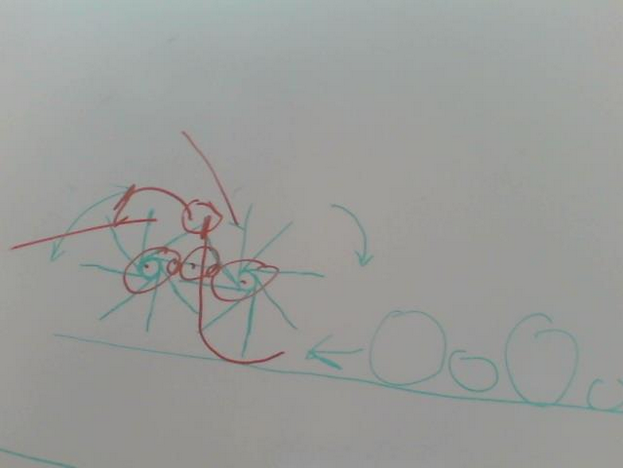
\includegraphics[width=10cm]{./Entries/Images/intake_device.png}
 % BatchedContinuous.png: 740x709 pixel, 90dpi, 20.89x20.01 cm, bb=0 0 592 567
\end{center}
The spinners represent brushes, but we are going to build the device with only one brush and test if it will work that way. The one-brush design will only use the front brush and have something to shove the ball up against (represented by the red line in between the two brushes).
